\newacronym{sts}{STS}{source and transport section}
\newacronym{sds}{SDS}{spectrometer and detector section}
\newacronym{wgts}{WGTS}{windowless gaseous tritium source}
\newacronym{dps}{DPS}{differential pumping section}
\newacronym{cps}{CPS}{cryogenic pumping section}
\newacronym{tlk}{TLK}{Tritium Laboratory Karlsruhe}
\newacronym{lara}{LARA}{laser Raman system}
\newacronym{bixs}{BIXS}{beta-induced X-ray spectroscopy}
\newacronym{fbm}{FBM}{forward beam monitor}
\newacronym{ckrs}{CKrS}{condensed \ce{^{83m}Kr} source}
\newacronym{mace}{MAC-E}{magnetic adiabatic collimation with electrostatic filtering}
\newacronym{emcs}{EMCS}{earth magnetic field compensation system}
\newacronym{lfcs}{LFCS}{low-field correction system}
\newacronym{vmms}{VMMS}{vertical magnetic measuring system}
\newacronym{rmms}{RMMS}{radial magnetic measuring system}
\newacronym{fpd}{FPD}{focal plane detector}
\newacronym{pulcinella}{PULCINELLA}{precision ultra-low current integrating normalization electrometer for low-level analysis}
\newacronym{ssc}{SSC}{source and spectrum calculation}
\newacronym{ft}{FT}{First Tritium}
\newacronym{knm1}{KNM1}{KATRIN Neutrino Mass Measurement 1}
\newacronym{mtd}{MTD}{measurement time distribution}
\chapter{The KATRIN Experiment}
    \section{Introduction}
    The KArlsruhe TRItium Neutrino (KATRIN) experiment performs a kinematic measurement of the tritium $\upbeta$ spectrum in order to determine the mass of the electron antineutrino (from here forth labeled $m_\nu$) as defined by equation (\ref{eq:nuMassSquared}). In case no neutrino mass signal is observed, KATRIN aims to set a an upper limit of
    \begin{equation*}
        m_\nu < \SI{200}{meV} \quad (\SI{90}{\percent} \text{ C.L.})
    \end{equation*}
    which is one order of magnitude lower than the one by its predecessor experiments. (See section \ref{sec:absoluteNuMassMeasurement}.)
    KATRIN recorded the first $\upbeta$ spectrum in March 2018 and started neutrino mass measurements in March 2019.
    
    \section{Experimental Setup}
    \begin{figure}[t]
        \inputpdftex{chapter/katrin/fig/beamline}
    	\xcaption{KATRIN beamline}{The KATRIN beamline.}{Main components from south to north:\\
    	a) rear section (see section \ref{sec:rearSection})\\
    	b) \glsentryfull{wgts} (see section \ref{sec:wgts})\\
    	c) \glsentryfull{dps} (see section \ref{sec:diffPumpingSection})\\
    	d) \glsentryfull{cps} (see section \ref{sec:cryoPumpingSection})\\
    	e) pre spectrometer (see section \ref{sec:spectrometer})\\
    	f) main spectrometer (see section \ref{sec:spectrometer})\\
    	g) detector (see section \ref{sec:detector})
    	}
	    \label{fig:beamline}
    \end{figure}
    The KATRIN experiment has a \SI{70}{m} beam line which is depicted in figure \ref{fig:beamline}. It can be divided into two sections: 
    \begin{enumerate}
        \item Within the \textbf{\gls{sts}} the tritium decays and the $\upbeta$ electrons are magnetically guided to the 
        \item \textbf{\gls{sds}} where they are filtered out according to their kinetic energy and finally counted at the detector.
    \end{enumerate}
    A comprehensive description of the KATRIN apparatus can be found in the KATRIN Design Report \cite{Angrik:2005ep} supplemented by more recent hardware overviews as e.g. in \cite{SeitzM2019}.
    
    Some central concepts of the source section are:
    {\par \textbf{Beam tube setup:} In the \gls{sts} the beam line is split into beam tube elements respectively stainless steel pipes. The pipes are either connected directly or by functional elements such as pump ports and valves.}
    
    {\par \textbf{Magnetic guidance of charged particles:} Superconducting coils surrounding the beam line in the \gls{sts} as well as coils around the spectrometer tank in the \gls{sds} create a magnetic field. The field lines are approximately parallel to the beam line and intersperse it over the range of the whole experiment. Charged particles perform cyclotron motions around the field lines and are adiabatically guided from the \gls{sts} to the detector. Adiabaticity is guaranteed by avoiding strongly varying field strengths on short distances.}
    
    {\par \textbf{Temperature:} Different parts and layers of the source section are operated at specific temperatures for several reasons such as establishing super-conductivity for the coils, stable gas dynamics and gas flow reduction. Several cooling systems based on liquid helium, neon, nitrogen and argon are installed. Additionally, in the \gls{sts}, the beam tube, the magnets and the hull are separated by insulation vacuums as well as heat shields of liquid nitrogen and neon.}
    
    {\par \textbf{Gas flow:} The spectrometer must be kept practically free of any tritium flow for safety and background reasons. Nonetheless, to allow an undisturbed passage of the $\upbeta$ electrons, the spectrometer is windowlessly connected to the source section. Hence, differential pumping sections are installed that reduce the inlet pressure of $\sim\SI{3e-3}{mbar}$ to the tritium partial pressure of the spectrometer of $\sim\SI{1e-11}{mbar}$.}
    
    \subsection{Windowless Gaseous Tritium Source}
    \label{sec:wgts}%
    \begin{figure}
        \centering
        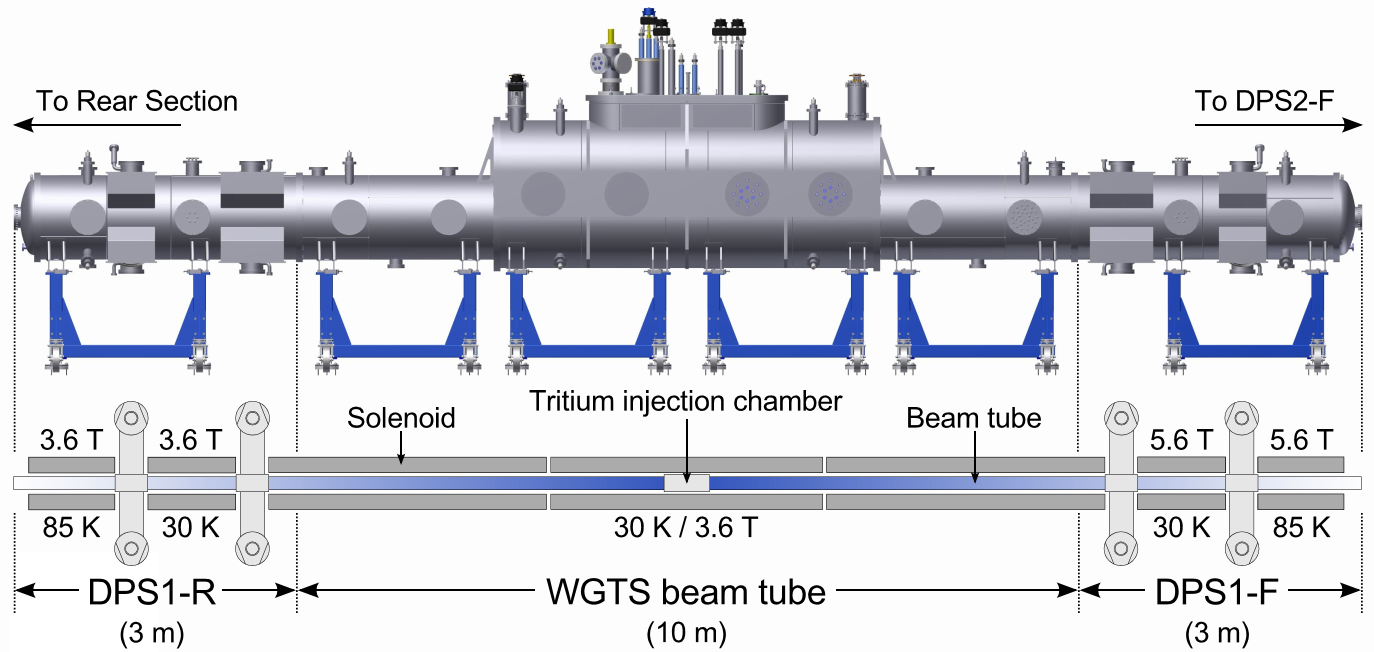
\includegraphics[width=\textwidth]{chapter/katrin/fig/wgts.png}
        \xcaption{KATRIN \glsentryfull{wgts}}{The \glsentryfull{wgts}.}{Shown are the hull and a sketch of the beam tube. Indicated are the molecular pumps, the design temperatures for tritium operation, the maximum magnetic field strengths and a color gradient depicting the decreasing gas density from the center to the sides. (From \cite{Harms2015})}
        \label{fig:wgts}
    \end{figure}%
The \gls{wgts} is a \SI{16}{m}-long, \SI{1.5}{m}-wide and \SI{4}{m}-high cryostat. It is depicted in figure \ref{fig:wgts} and a detailed description can e.g. be found in \cite{Grohman2008}.
    {\par \textbf{The inner loop:} The molecular tritium (\ce{T2}) is injected centrally in the \gls{wgts}'s \SI{90}{mm}-wide beam tube where it decays. The design gas column density is 
    \begin{equation}
        \label{eq:columnDensity}
        \rho d = \SI{5e17}{molecules/{cm}^2}
    \end{equation}
    of which \begin{equation}
        \epsilon_\text{T} = \SI{95}{\percent}
    \end{equation}
    are isotopic tritium molecules. At the front and rear of the \gls{wgts} the gas is extracted from the beam tube by molecular pumps in designated differential pumping sections called DPS-1-R (rear) and DPS-1-F (front). The extracted gas is re-injected in the center of the beam tube. The respective pipe system is called the inner loop.
    \begin{samepage}
    Selected important parts of the inner loop are:
    \begin{itemize}
    \renewcommand{\labelitemi}{$\bullet$}
        \item a buffer vessel where tritium of high purity is introduced from the feed loop of the \gls{tlk};
        \item a \gls{lara} that monitors the isotopic composition of the gas;
        \item a pressure and temperature controlled buffer vessel to regulate the gas inlet into the \gls{wgts}; and
        \item a permeator that separates impurities (like e.g. helium) and ejects them into the exhaust loop of the \gls{tlk}.
    \end{itemize}
    \end{samepage}}
    
    
    {\par\textbf{Magnetic field:}
    In order to adiabatically guide the $\upbeta$ electrons to the spectrometer section the \gls{wgts} is submerged in a magnetic field parallel to its beam tube of up to \SI{5.6}{T}. It is created by 7 superconducting coils, that surround the beam tube. These magnets are kept at a temperature of \SI{4.2}{K} by liquid helium.}
    
    {\par\textbf{Temperature:}
    The stability of the column density \eqref{eq:columnDensity} must be on the \SI{0.1}{\percent} level. This requires stable parameters like temperature $T$ and pressure $p$. On one hand, the higher the temperature the less stable the system. Furthermore, thermal motion smears the energy spectrum of the $\upbeta$ electrons (Doppler effect). On the other hand, at low temperatures the gas molecules cluster. $T=\SI{30}{K}$ is chosen as a compromise and established by a two-phase neon cooling system. For calibration purposes it is also possible to operate the \gls{wgts} with krypton instead of tritium. This requires a beam tube temperature of $T=100K$ in order for the krypton not to freeze. In this operational mode the neon has to be exchanged for argon that provides a suitable vapor pressure.}
    
    \subsection{Rear Section}
    \label{sec:rearSection}
    \begin{figure}[t]
        \inputpdftex{chapter/katrin/fig/rear-section}
    	\xcaption{KATRIN rear section}{The rear section}{terminates the KATRIN beam line and houses several monitoring and calibration devices. (Adapted from \cite{SeitzM2019})}
	    \label{fig:rearSection}
    \end{figure}
    
    The rear section terminates the beam line in the upstream direction. It houses monitoring, calibration and control devices. It is depicted in figure \ref{fig:rearSection} and a detailed description can e.g. be found in \cite{Babutzka2014}.
    
    {\par \textbf{Rear wall:} The so-called rear wall is a gold-coated stainless-steel disc with a diameter of 6 inches that terminates the beam tube.}
    
    {\par\textbf{Electron gun:}
    The rear section houses an electron gun in order to measure the response function of the experiment (see section \ref{sec:response}). Its energy resolution is $\sim \SI{0.2}{eV}$ and its angular resolution is $\sim \SI{4}{\degree}$. The electrons' flight path can be adjusted by dipole magnets mounted in the \gls{wgts} which enables a scanning of the full beam tube.}
    
    {\par\textbf{Plasma control:}
    Space charges, respectively a plasma, forms within the \gls{wgts} due to the tritium decay. $\upbeta$ electrons might therefore start at different potentials which adds uncertainty to the measured $\upbeta$ spectrum. Hence, plasma effects have to be controlled. Simulations show that the plasma can be influenced by the rear wall potential which can be controlled by a voltage supply in the range of $\pm \SI{10}{V}$. Moreover, a UV light illumination of the rear wall can extract electrons via the photoelectric effect that can compensate space charges. Details on the plasma in the \gls{wgts} can e.g. be found in \cite{Kuckert2018}.}
    
    {\par\textbf{Activity monitoring:}
    $\upbeta$ electrons either arrive at the detector or hit the wall of the experiment. A super conducting coil ensures that the magnetic flux tube terminates at the rear wall. On that account, most $\upbeta$ electrons (\SI{99.99}{\percent}) hit the rear wall where they emit bremsstrahlung. Two dedicated \gls{bixs} systems measure the corresponding X-ray spectrum to determine the source strength respectively the gas column density \eqref{eq:columnDensity}.}
    
    \subsection{Differential Pumping Section}
    \label{sec:diffPumpingSection}
    \begin{figure}[t]
        \inputpdftex{chapter/katrin/fig/dps}
    	\xcaption{KATRIN \glsentryfull{dps}}{The \glsentryfull{dps}}{reduces the gas flow and blocks tritium ions. (Adapted from \cite{SeitzM2019})}
	    \label{fig:dps}
    \end{figure}
    The \glsentryfull{dps} is an approximately \SI{5}{m}-long cryostat. It is depicted in figure \ref{fig:dps} and a detailed description can e.g. be found in \cite{Kosmider2012}. In short, it fulfills the following tasks:
    
    {\par\textbf{Reduction of tritium flow:}
    The \glsentryfull{dps} consists of 5 beam tube elements with pump ports between them. The beam tube elements form a \SI{20}{\degree} angle to each other and are arranged in a chicane. While $\upbeta$ electrons are magnetically guided along the chicane, the neutral gas molecules scatter off the walls. This reduces the molecular beaming effect and enhances the pumping probability. Turbo molecular pumps then reduce the gas flow by approximately 5 orders of magnitude and feed the gas into the so-called outer loop where it is reprocessed.}
    
    {\par\textbf{Ion blocking:}
    In the \gls{wgts} ions such as \ce{HeT^+}, \ce{T_2+}, \ce{T_3+}, \ce{T_5+} can form. If not blocked, they reach the spectrometer section analogously to the electrons which would eventually lead to an increased background rate. A potential barrier created by two ring electrodes set to $+\SI{100}{V}$ avoids this. The positive ions are deflected, drift out of the flux tube, hit the wall and get neutralized.}
    
    {\par\textbf{Ion monitoring:}
    Downstream of the blocking electrodes the remaining ion flux is measured by a Fourier transform ion cyclotron resonance device (FT-ICR). Details on ion forming and their measurement can e.g. be found in \cite{Ubieto2009}.}
    
    \subsection{Cryogenic Pumping Section}
    \label{sec:cryoPumpingSection}
    \begin{figure}[t]
        \inputpdftex{chapter/katrin/fig/cps}
    	\xcaption{KATRIN \glsentryfull{cps}}{The \glsentryfull{cps}}{is the coldest part of the KATRIN experiment. Parts of its beam tube a covered by a frozen argon layer at \SI{3}{K} to cold-trap tritium molecules. The low temperatures are established using liquid helium (\ce{LHe}) and an insulation of liquid nitrogen (\ce{LN2}). (Adapted from \cite{SeitzM2019})}
	    \label{fig:cps}
    \end{figure}
    
    The \glsentryfull{cps} is an approximately \SI{7}{m}-long cryostat. It is depicted in figure \ref{fig:cps} and a detailed description can e.g. be found in \cite{Jansen2015}. In short, it fulfills the following tasks:
    {\par\textbf{Reduction of tritium flow:}
    The \gls{cps} consists of 7 beam tube elements of which 5 are arranged in a similar manner as the beam tube elements of the \gls{dps} in a chicane forming \SI{15}{\degree} angles. While charged particles are guided along the chicane by a magnetic field, neutral molecules hit the wall. The walls are covered by a frozen argon layer cooled down to \SI{3}{K} in order to cold-trap particles. After the accumulation of about \SI{1}{Ci} of tritium the argon frost layer has to be renewed. To achieve this the beam tube is warmed-up and the argon is pumped off along with the accumulated tritium. Tests and simulations show a reduction of the tritium flow by approximately 10 orders of magnitude.}

    {\par\textbf{The \glsentryfull{fbm}}: The \glsentryshort{fbm} is a detector that can be moved horizontally into the pump port of the \gls{cps} with a 2-dimensional spacial resolution of \SI{0.1}{mm}. Two pin-diodes measure the $\upbeta$ electron flux and hence, the stability of the column density \eqref{eq:columnDensity}. Furthermore, the \gls{fbm} equips a temperature and a hall sensor. A second detector board holding a Faraday cup for ion measurements is also available. Details on the \gls{fbm} can e.g. be found in \cite{Ellinger2017}.}
    
    {\par\textbf{The \glsentryfull{ckrs}} is a sub mono-layer of \kryptonEightyThree{} on a pyrolytic graphite substrate with a diameter of \SI{2}{cm}. It can be lowered in the pump port of the \gls{cps} and moved in a 2-dimensional plane perpendicular to the beam line. This enables the spacial scanning of the properties of the spectrometer using quasi-monoenergetic conversion electron lines of \kryptonEightyThree. Details on the \glsentryshort{ckrs} can e.g. be found in \cite{Bauer2014}.}
    
    \subsection{Pre and Main Spectrometer}
    \label{sec:spectrometer}
    
    The pre and main spectrometer are vacuum vessels designed to filter passing electrons according to their kinetic energy. The pre spectrometer has a length of \SI{3.4}{m} and a diameter of \SI{1.7}{m}. Details on its design can e.g. be found in \cite{Prall2012}. The main spectrometer has a length of \SI{23}{m} and a diameter of \SI{10}{m}. Details on its design can e.g. be found in \cite{Angrik:2005ep}.
    
    {\par \textbf{\Gls{mace}}: The pre and main spectrometer apply the so-called \glsentryshort{mace} principle. A retarding voltage deflects electrons with insufficient kinetic energy. The electric field gradient is parallel to the beam line, but $\upbeta$ electrons might be emitted in an arbitrary angle. In order to analyze their full kinetic energy they have to be collimated. This is done by a magnetic field gradient. A quantitative description of this process can be found in section \ref{sec:intSpecModel}. The precision of the \gls{mace} principle increases with the size of the spectrometer. That is why the main spectrometer of KATRIN has a larger diameter (\SI{10}{m}) as the the ones of its predecessor experiments.
    }
    
    {\par \textbf{Magnetic field:} The main spectrometer is surrounded by a system of coils that creates the \gls{mace} filter's  magnetic field. Upstream, there is the PS2 magnet; downstream the pinch as well as the detector magnet, which are superconducting solenoids. Their field is fine-tuned by a system of air coils around the spectrometer hull. There is the \gls{emcs} with coils parallel and perpendicular to the beam line axis. Furthermore, there is the \gls{lfcs} with coils perpendicular to the beam line axis. The combined system constrains the electrons' flux tube to the spectrometer vessel and compensates the earth's magnetic field as well as effects from ferromagnetic materials in the spectrometer's surroundings. Details on the magnetic field settings can e.g. be found in \cite{Erhard2018}. Additionally, a vertical and radial magnetic measuring system (\glsentryshort{vmms} and \glsentryshort{rmms}) are installed. The field inside the spectrometer vessel is assessed via samples of these measuring systems combined with simulations. Details on the \glsentryshort{vmms} and the \glsentryshort{rmms} can e.g. be found in \cite{Letnev2018}.}
    
    {\par \textbf{Electric field:} A high voltage system establishes the \gls{mace} filter's retarding potential. According to the KATRIN Design Report \cite{Angrik:2005ep} the retarding voltage's fluctuations must have a standard deviation smaller than \SI{60}{mV} for the envisaged sensitivity on the neutrino mass. The antenna-like beam line setup is sensitive to electromagnetic fluctuations, which is why an active so-called post-regulation system is deployed. It monitors the retarding potential and regulates it with the needed precision. For the monitoring exist the so-called monitor spectrometer and a voltage divider. Details on the voltage calibration with the voltage divider can e.g. be found in \cite{Thuemmler2009}. The monitor spectrometer is part of a second beam line in a separate building. Its retarding potential follows the one one of the main spectrometer and is measured via \kryptonEightyThree{} conversion lines. Details on the monitor spectrometer can be e.g. be found in \cite{Erhard2014}.}
    
    {\par \textbf{Background:} According to the KATRIN Design Report \cite{Angrik:2005ep} the electron rate of uncontrollable sources (background) must be less than \SI{10}{mHz}. Several background-related aspects are:}
    
    {\par \textbf{Vacuum:} The spectrometers are operated at a pressure on the order of \SIrange{10e-11}{10e-12}{mbar}. This prevents electron scattering on residual gas and minimizes background effects by ionization. Correspondingly, several turbo molecular and getter pumps are installed at the spectrometer vessels. Furthermore, the spectrometers can be baked out at up to \SI{350}{\celsius}. Details on the vacuum system can e.g. be found in \cite{Arenz2016}.}
    
    {\par \textbf{Wire electrodes:} The inner walls of the spectrometer vessels are lined by wire electrodes. Their potential is at a few hundred volts below the spectrometer hull reflecting electrons coming from the vessel walls. These electrons might be induced by e.g. cosmic rays or emanate from the spectrometer wall. A detailed description of the wire electrodes can e.g. be found in \cite{Valerius2009}.}
    
    {\par \textbf{Ion blocking:} Analogously to the ones in the \gls{cps} (section \ref{sec:cryoPumpingSection}), three blocking electrodes are installed; one between the \gls{cps} and the pre spectrometer, one between the pre and main spectrometer; and one between the main spectrometer and the detector.}
    
    {\par \textbf{Tandem setup:} $\upbeta$ electrons might scatter on residual gas or the beam line walls. This can either directly lead to secondary electrons or create positive ions that travel down the beam line. The positive ions in turn might again through scattering yield secondary electrons. The more $\upbeta$ electrons enter the main spectrometer the higher is the probability to create secondary electrons. In order to reduce the flux of $\upbeta$ electrons into the main spectrometer the retarding potential of the pre spectrometer is set to a few hundred volts below the one of the main spectrometer. On one hand this is a countermeasure against background events. But on the other hand, charged particles can be trapped between the two spectrometers due to the electromagnetic setup (Penning trap). A sudden discharge might harm the hardware, especially the detector. Therefore, it is possible to sweep a charged wire through the volume in order to collect the trapped particles and avoid this ``Penning-discharges''.}
    
    \subsection{Detector Section}
    \label{sec:detector}
    \begin{figure}[t]
        \inputpdftex{chapter/katrin/fig/detector-section}
    	\xcaption{KATRIN detector section}{The detector section}{terminates the KATRIN beam line. Among other instruments it houses the \glsentrylong{fpd} for $\upbeta$ electrons with the detector wafer at its core.(Adapted from \cite{SeitzM2019})}
	    \label{fig:detector}
    \end{figure}
    
    The detector section terminates the beam line in downstream direction. It can be separated from the spectrometer section by closing a gate valve. The detector section is depicted in figure \ref{fig:detector} and a detailed description can e.g. be found in \cite{Amsbaugh2015}.
    
    {\par \textbf{The \gls{fpd}} counts the $\upbeta$ electrons that pass the spectrometer section. The \gls{fpd} is a pin-silicon detector with a sensitive area of \SI{9}{cm} diameter. It is subdivided in 148 pixels of the same area arranged in 12 rings of 12 pixels each and the so called bull's eye of 4 pixels in the center. This arrangement allows later correction for radial electrical and magnetic inhomogeneities in the beam line.}
    
    {\par \textbf{Shield and veto system:} The \gls{fpd} system's radiation shield consists of two nested cylindrical shells: an outer lead shell of \SI{3}{cm} that reduces photon background and an inner copper shell of \SI{1.27}{cm} that blocks X-rays originating from the outer lead shell. The shield is surrounded by a veto system to tag incoming muons.}
    
    {\par \textbf{Calibration:} Photoelectron sources can be lowered in the detectors line of sight. The corresponding photocurrent can be measured with the so-called \gls{pulcinella} system. A comparison of \gls{pulcinella} and the \gls{fpd} yields the \gls{fpd}'s detection efficiency.}
    
    {\par \textbf{The detector magnet} allows to form the flux tube near the detector independently of the main spectrometer magnetic field setting. This is especially useful in the above mentioned calibration process.}
    
    {\par \textbf{The post-acceleration electrode} allows to shift the energy of $\upbeta$ electrons arriving from the main spectrometer. This way $\upbeta$ electrons can be distinguished from background electrons originating in the detector section by an energy region of interest cut.}
    
   \newcommand{\elecIndex}{\mathrm{e}}
\newcommand{\fermiConst}{G_\mathrm{F}}
\newcommand{\diffRate}{\frac{\d\Gamma}{\d E}}
\newcommand{\nucMatrixElement}{M_\mathrm{nuc}}
\newcommand{\thetaFunc}{\Theta}

\newcommand{\Bsource}{B^j_\mathrm{S}}
\newcommand{\zSource}{z_\mathrm{S}}
\newcommand{\thetaSource}{\theta_\mathrm{S}}
\newcommand{\Esource}{E_\mathrm{S}}
\newcommand{\Usource}{U^j_\mathrm{S}}
\newcommand{\gammaSource}{\gamma_\mathrm{S}}


\newcommand{\Bps}{B_\mathrm{PS2}}
\newcommand{\Bana}{B_\mathrm{A}}
\newcommand{\Bpinch}{B_\mathrm{P}}
\newcommand{\Bmax}{B_\mathrm{max}}
\newcommand{\Bmin}{B_\mathrm{min}}

\newcommand{\thetaMax}{\theta_\mathrm{max}}
\newcommand{\Esur}{E_\mathrm{sur}}
\newcommand{\detEff}{\epsilon_\mathrm{det}}
\newcommand{\macefilterwidth}{\Delta \mathcal{E}^j(\thetaS^j)}

\newcommand{\EtransPure}{E^j_\mathrm{tr}}
\newcommand{\Etrans}{\EtransPure(qU,\Esource,\thetaSource)}
\newcommand{\thetaTransPure}{\theta^j_\mathrm{tr}}
\newcommand{\thetaTrans}{\thetaTransPure(\Esource,qU)}

\newcommand{\As}{A_\mathrm{S}}
\newcommand{\Rbg}{R_\mathrm{bg}}


\section{Modelling of the Integrated \texorpdfstring{$\upbeta$}{Beta} Decay Spectrum with SSC}
\label{sec:intSpecModel}
An analytic description for the electron rate measured by the \gls{fpd} can be derived. The derivation mostly follows \cite{Kleesiek2019, Groh2015, Kleesiek2014} or is extracted from current production code \cite{KATRINCOL2019}. The formulas are implemented in the so-called \gls{ssc} software framework.

\subsection{\texorpdfstring{$\upbeta$}{Beta} Decay Spectrum}
\begin{figure}
    \centering
    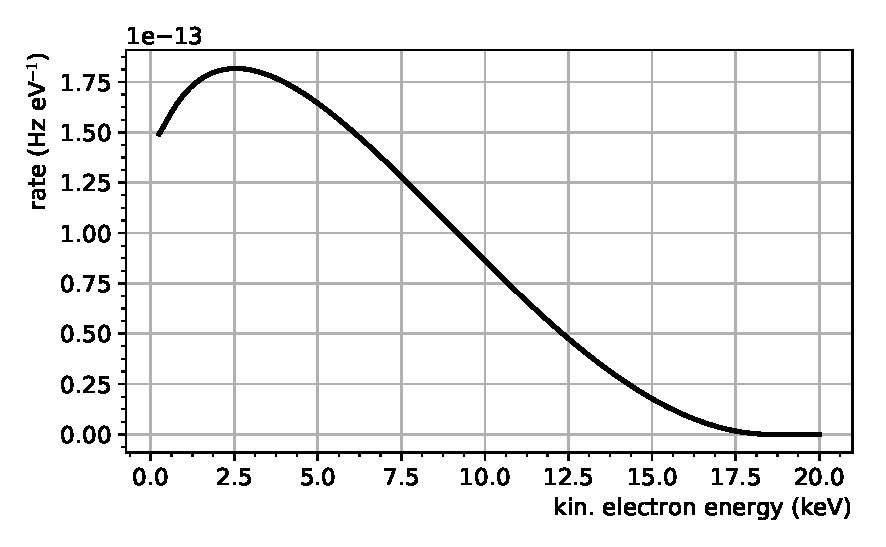
\includegraphics[width=\textwidth]{chapter/katrin/fig/diffSpec.pdf}
    \xcaption{Tritium $\upbeta$ spectrum}{The $\upbeta$ decay spectrum of a tritium molecule}{as calculated by \gls{ssc}.}
    \label{fig:diffSpec}
\end{figure}
\label{sec:diffSpec}
In $\upbeta^-$ decay the released energy is distributed among the emitted electron and the anti-electron neutrino. The differential decay rate of a tritium molecule can be described using Fermi theory and Fermi's golden rule as
\begin{align}
    \label{eq:diffRate}
    \left(\diffRate\right) = &
    \frac{\fermiConst^2 \abs{V_\mathrm{ud}}^2}{2 \pi^3}
    \abs{\nucMatrixElement}^2 \cdot
    F(Z, E) \cdot 
    p(E+m_\elecIndex) \cdot 
    \sum_{f,i} P_f \abs{U_{\elecIndex i}}^2 \epsilon_f \sqrt{\epsilon_f^2-m_i^2} \cdot \thetaFunc(\epsilon_f-m_i)
\end{align}
It is depicted in figure \ref{fig:diffSpec}. Its constituents are the kinetic electron energy $E$;
the PMNS matrix $U$ \eqref{eq:PMNSmatrix}; the neutrino eigenmasses $m_i$ \eqref{eq:nuMassSquared};
the Fermi constant $\fermiConst$;
the up-down-quark-coupling given by the Cabibo angle $\theta_\mathrm{C}$
\begin{equation}
    V_\mathrm{ud} = \cos \theta_\mathrm{C} = 
    0.97425\pm0.00022;
\end{equation}
and the nuclear transition matrix element
\begin{equation}
    \nucMatrixElement = g_V^2+3g_A^2 \quad
    \text{with } g_v = 1 \quad
    \text{and} \quad g_A/g_V = -1.2646 \pm 0.0035
\end{equation}
which is independent of the electron's kinetic energy as the decay is super-allowed and given by the vector $g_V$ and axial vector $g_A$ coupling.

Furthermore, the Fermi function $F(Z,E)$ accounts for the Coulomb interaction between the outgoing electron and the daughter nucleus with atomic charge $Z=2$ which in its relativistic version can be approximated as
\begin{equation}
    F(Z,E) \approx \frac{2 \pi \eta}{1-\exp{2 \pi \eta}} \cdot R \\
\end{equation}
with Sommerfeld parameter $\eta = \alpha Z / \beta$, fine structure constant $\alpha$, relativistic velocity $\beta$ and a relativistic correction factor $R = 1.002037-0.001427\beta$.

The phase-space factor of the outgoing electron with momentum $p$ and mass $m_\elecIndex$ is given by the factor $p(E+m_\elecIndex)$.

The phase space factor of the emitted neutrino is described in dependence of the following quantities: total nuclear tritium decay energy $Q$ (mass difference of mother and daughter nucleus) corrected for the nucleus recoil $E_\mathrm{rec}$ also called endpoint of the $\upbeta$ spectrum
\begin{equation}
    \label{eq:endpoint}
    E_0 = Q-E_\mathrm{rec};
\end{equation}
the kinetic electron energy $E$ and the final state energy of the molecular system $V_f$. The probability that the molecular system is in a final state of energy $V_f$ after the decay is denoted by $P_f$. Then the energy of the neutrino reads 
\begin{equation}
    \epsilon_f = E_0 - E - V_f \fullstop
\end{equation}

The exited energy state $f$ is caused by vibration, rotation or electronic excitation of the decaying molecule. Details and tabulated values can e.g. be found in \cite{Bodine2015} and references therein.

The neutrino's momentum is $\sqrt{\epsilon_f^2-m^2_i}$, where $m_i$ denotes one of the neutrino eigenmasses. The complete phase space factor of the neutrino is a sum over all possible molecular final states labeled $f$ and neutrino eigenmasses labeled $i$.

Lastly, the Heavyside step function $\thetaFunc$ ensures a positive kinetic energy of the neutrino.

\subsection{Detector Counts}
The KATRIN detector counts electrons. The $\upbeta$ electrons are adiabatically guided from the \gls{wgts} to the detector by magnetic fields. The magnetic field lines are parallel to the beam line axis. The angle between the flight direction of a $\upbeta$ electron and the beam line axis towards the detector is denoted by the pitch angle $\theta \in [\SI{0}{\degree}, \SI{180}{\degree}]$. The starting position of an $\upbeta$ electron is denoted by its 1-dimensional coordinate along the beam line axis $\zSource$. 

KATRIN measures an integrated $\upbeta$ spectrum. In other words, the detector counts electrons of kinetic energy $\Esource$ above a threshold, the so-called retarding energy $qU$. The integrated $\upbeta$ spectrum can be scanned by varying $qU$.

A $\upbeta$ electron emitted in the \gls{wgts} reaches the detector with a probability modeled by the so-called response function $R$ (see section \ref{sec:response}). $R$ depends on the experimental settings (such as the electromagnetic fields and the gas dynamics) and especially on the retarding energy $qU$. Here, $R$ denotes the transmission probability for a $\upbeta$ electron of a fixed starting kinetic energy $\Esource$, starting position $\zSource$ and starting pitch angle $\thetaSource$. The probability of a $\upbeta$ electron for being counted when reaching the detector is denoted by the detection efficiency $\detEff$. Furthermore, the number of tritium molecules in the \gls{wgts} in a small area around the coordinate $z$ is denoted by $\d N_T(z)$. 

Then, the measured integrated rate is expressed as integral from the threshold energy $qU$ to the endpoint energy $E_0$ \eqref{eq:endpoint} over the differential rate $\d \Gamma / \d \Esource$ \eqref{eq:diffRate} weighted with the probability given by $R$ as
\begin{equation}
\label{eq:rateDependingOnstartingValues}
\Gamma(qU, \zSource, \thetaSource) = 
\detEff \cdot
\d N_T(\zSource) \cdot
\int_{qU}^{E_0} 
    \left(\frac{\d \Gamma(\Esource)}{\d \Esource}\right) \cdot 
    R(\Esource, qU, \zSource, \thetaSource) 
\d \Esource
\comma
\end{equation}
which eventually leads to $\upbeta$ electron counts by multiplication with the measurement time $t(qU)$ at a retarding energy $qU$
\begin{equation}
    \label{eq:countsDependingOnPositionAndPitchAngle}
    N(qU, \zSource, \thetaSource) = \Gamma(qU, \zSource, \thetaSource) \cdot t(qU)
    \fullstop
\end{equation}

\subsection{Discretization of the \glsentryshort{wgts} Volume}
\label{sec:sourceDiscretization}
The counts $N$ \eqref{eq:countsDependingOnPositionAndPitchAngle} are given for $\upbeta$ electrons of a fixed starting position $\zSource$.
All starting positions $\zSource \in [-L/2, +L/2]$ within the \gls{wgts} of length $L$ contribute to the total count rate at the detector. Integrating along the beam axis accounts for this
\begin{equation}
    N(qU, \thetaSource) = \int_{-L/2}^{+L/2} \frac{\d N(qU, \thetaSource, \zSource)}{\d \zSource} \d \zSource
\end{equation}
Numerically, the same result can be obtained by a sufficiently fine discretization of the \gls{wgts} volume into $S$ slices. The counts $N$ \eqref{eq:countsDependingOnPositionAndPitchAngle} are adapted accordingly to account for discrete starting $\upbeta$ electron positions $\zSource^j$
\begin{equation}
    N(qU, \thetaSource, \zSource) \rightarrow N^j(qU, \thetaSource,\zSource^j) \equiv N^j(qU, \thetaSource) \fullstop
\end{equation}
Then, the total counts read
\begin{equation}
    \label{eq:nonAveragedCounts}
    N(qU, \thetaSource) = \sum_{j=1}^S N^j(qU, \thetaSource) \fullstop
\end{equation}
Within this chapter, from here forth all quantities that are subject to discretization will be labeled with an upper index $j$. The discretization especially propagates to the response function $R \rightarrow R^j$ and its constituents.

\subsection{Magnetic Bottle Effect}
The $\upbeta$ electrons are adiabatically guided to the detector by magnetic fields. The magnetic field strength at the starting position of a $\upbeta$ electron in the \gls{wgts} is denoted by $\Bsource$. The maximum magnetic field strength along the beam line is denoted by $\Bmax$. As $\Bsource<\Bmax$ $\upbeta$ electrons travelling downstream to the detector are subject to the magnetic bottle effect. They get reflected and travel upstream to the rear wall if their starting pitch angle $\thetaSource$ surpasses $\thetaMax^j$ with
\begin{equation}
    \label{eq:thetaMax}
    \sin\thetaMax^j = \sqrt{\frac{\Bsource}{\Bmax}} \fullstop
\end{equation}
(Its KATRIN design value is $\thetaMax\approx \SI{51}{\degree}$.) A cutting angle $\thetaMax^j$ is beneficial because the greater the emission angle of a $\upbeta$ electron the larger the distance it travels in the \gls{wgts} and the more it is subject to energy losses such as scattering or synchrotron radiation.

\subsection{Scattering Probabilities}
\label{sec:scatProbs}
The probability for a $\upbeta$ electron to reach the detector (the response function $R^j$) depends on the scattering probabilities $P_l$ ($l \in \NN$). $P_l$ denotes the probability of an electron to scatter $l$ times when travelling through the \gls{wgts}. $P_l$ depends on the starting position $\zSource$ of a $\upbeta$ electron in the \gls{wgts} as well as on its starting pitch angle $\thetaSource$. The expected scattering count for a $\upbeta$ electron when travelling through the \gls{wgts} is the product of the line density $\lambda$ the electron passes through and the scattering cross section $\sigma$
\begin{equation}
    \label{eq:expectedScatteringCount}
    \mu(\zSource, \thetaSource) = \lambda(\zSource,\thetaSource) \sigma \fullstop
\end{equation}
The electron moves on a spiral due to its cyclotron motion. Therefore, when traveling an infinitesimal distance $\d z$ in $z$-direction, it travels a total distance of
\begin{equation}
    \label{eq:infinitesimalElecPath}
    \d s = \frac{1}{\cos\thetaSource} \d z \fullstop
\end{equation}
The line density $\lambda$ can be expressed as a line integral over the gas density $\rho$ along the electrons path $\varphi$
\begin{equation}
    \label{eq:lambdaPath}
    \lambda(\zSource,\thetaSource) = \int_{\varphi} \rho(\Vec{r})\d s
    \fullstop
\end{equation}
Assuming that the gas density $\rho$ only depends on the $z$-position along the beam line and vanishes for $z>L/2$ (beyond the \gls{wgts}) equation (\ref{eq:lambdaPath}) becomes
\begin{equation}
    \label{eq:lambdaPathIntegral}
    \lambda(\zSource,\thetaSource) = \frac{1}{\cos\thetaSource}\int_{\zSource}^{L/2} \rho(z)\d z \fullstop
\end{equation}
Hence, the expected scattering count (\ref{eq:expectedScatteringCount}) becomes
\begin{equation}
    \label{eq:expectedScatRate}
    \mu(\zSource, \thetaSource) = \frac{\sigma}{\cos\thetaSource}\int_{\zSource}^{L/2} \rho(z)\d z \fullstop
\end{equation}
The scattering process fulfills the conditions of a Poisson process, namely scattering once does quasi not influence the probability of an electron to scatter again; the expected scattering count $\mu$ \eqref{eq:expectedScatRate} stays quasi constant; and it is unlikely for two scatterings to happen within a short distance. Thus, the probability for $l$-fold scattering can be expressed as a Poisson distribution
\begin{equation}
    \label{eq:scatProbs}
    P_l(\zSource, \thetaSource) = 
    \frac{
        \mu(\zSource, \thetaSource)^l
    }{l!}
    \mathrm{e}^{-\mu(\zSource, \thetaSource)} \fullstop
\end{equation}
\paragraph{Discretization of the \gls{wgts} volume}
In the discretized case the \gls{wgts} volume is divided into $S$ slices indexed by $k$ with an average gas density $\bar{\rho}^k$. A slice $k$ starts at position $Z_s^k$ and ends at position $Z_e^k$ with a width of $W^k=Z_e^k-Z_s^k$. For $\upbeta$ electrons that start at a position $z$ within slice $j$ the expected scattering count \eqref{eq:expectedScatteringCount} becomes
\begin{equation}
\label{eq:nonAveragedExpectedScatCount}
    \mu(\zSource, \thetaSource) \rightarrow 
    \mu^j(z, \thetaSource) =
    \frac{\sigma}{\cos\thetaSource}
    \underbrace{
        (Z_e^j-z) \bar{\rho}^j
        \vphantom{\sum_{k=j+1}^{S}}
    }_{(*)}
    \underbrace{\sum_{k=j+1}^{S} \bar{\rho}^k W^k}_{(**)}
    \fullstop
\end{equation}
The gas column density in front of a $\upbeta$ electron is split in two parts: the slice of its \mbox{origin $(*)$} and all slices downstream \mbox{$(**)$}. 

The Poisson distribution is formed for the expected scattering count $\mu^j$ \eqref{eq:nonAveragedExpectedScatCount} and averaged over all starting positions within the slice $j$ which yields the discretized scattering probabilities
\begin{equation}
    \label{eq:nonAveragedScatProbs}
    P^j_l(\thetaSource) = 
    \frac{1}{W^j}
    \int_{Z_s^j}^{Z_e^j}
        \frac{
            \left(\mu^j(z,\thetaSource)\right)^l
        }{l!}
        \mathrm{e}^{-\mu^j(z,\thetaSource)}
    \d z
    \fullstop
\end{equation}


\subsection{\glsentryshort{mace} Principle and Transmission Function}
\label{sec:mace}
\begin{figure}[t]
        \inputpdftex{chapter/katrin/fig/mace}
    	\xcaption{Schematic of the KATRIN main spectrometer and the \glsentryshort{mace} principle.}{
    	Schematic of the KATRIN main spectrometer and the \glsentryfull{mace} principle.}{
    	 The {KATRIN} design magnetic field settings are
    	$\Bps=\SI{4.5}{T}$, 
    	$\Bsource=\SI{3.6}{T}$, 
    	$\Bmax=\SI{6.0}{T}$, 
    	$B_\mathrm{D}=\SI{3.6}{T}$, 
    	$\Bana\approx\SI{3e-4}{T}$. $\Vec{E}$ denotes the magnetic field regulated by the retarding potential $U$ that reaches its maximum $U_\mathrm{a} = U$ at the analyzing plane. (Adapted from \cite{SeitzM2019})
    	}
	    \label{fig:mace}
    \end{figure}

The spectrometers of KATRIN follow the \glsentryfull{mace} principle. Figure \ref{fig:mace} shows a corresponding sketch. The main spectrometer is a vacuum vessel with a downstream magnet of strength $\Bps$ and an upstream magnet of strength $\Bpinch$ making electrons form a magnetic flux tube. In the case of KATRIN the fluxtube begins in the \gls{sts} with a magnetic field strength of $\Bsource$. In other words, the spectroscopic properties are not solely determined by the spectrometer vessel, but also by the \gls{sts}. The minimum magnetic field strength $\Bmin = \Bana$ is reached at the so-called analyzing plane in the vessel center. Electrons entering the vessel perform cyclotron motions around the magnetic field lines. Their total kinetic energy $\Esource$ is split into a longitudinal component $E_\parallel$ along the beam axis and a transverse component $E_\bot$
\begin{equation}
    \label{eq:totalKinElecEnergy}
    \Esource = E_\parallel + E_\bot \fullstop
\end{equation}
In the non-relativistic and adiabatic approximation the transverse component can be expressed by the magnetic field strength $B$ and the electron's magnetic moment $\mu$ respectively its charge $q=e$, its mass $m_\elecIndex$ and angular momentum $L$.
\begin{equation}
    E_\bot = - \mu B = \frac{e}{2 m_\elecIndex}LB \fullstop
\end{equation}
Adiabaticity conserves angular momentum $L$ and the total energy of the electron $\Esource$. Hence, when the magnetic field strength $B$ decreases to $\Bana=\Bmin$ in the analyzing plane, the transverse component of the electron's energy $E_\bot$ decreases likewise and transforms to longitudinal energy $E_\parallel$. Additionally, a retarding voltage barrier is applied along the beam axis, reaching its maximum $U$ at the analyzing plane and dropping of towards the source and the detector. 
In order to pass through the filter, electrons need a total kinetic energy $\Esource$ greater than the transmission energy $\Etrans$ that depends on their starting potential $\Usource$, their starting pitch angle $\thetaSource$ and starting Lorentz factor $\gammaSource$
\begin{equation}
    \label{eq:transmissionEnergy}
    \Etrans = 
    \frac{
        q(U-\Usource)
    }{
        1-\sin^2\thetaSource \frac{\Bana}{\Bsource} \frac{\gammaSource+1}{2}
    }
    \fullstop
\end{equation}
For ease of notation, the dependency on $\Bsource$, $\Bana$ and $\Usource$ is left implicit. Note further that the right hand side of \eqref{eq:transmissionEnergy} also depends on the starting energy of a $\upbeta$ electron as it depends on $\gammaSource$.

Then, the probability for an electron to pass through a \gls{mace} filter, the so-called transmission function, can be written as
\begin{equation}
    \label{eq:transmissionWithConditionOnEnergy}
    \mathcal{T}^j(\Esource, qU, \thetaSource) =
    \begin{cases}
    1 & \text{if } \Esource > \Etrans \\
    0 & \text{otherwise} 
    \end{cases}
    \fullstop
\end{equation}

The transmission condition for the energy $\Esource > \Etrans$ can be reformulated to a condition for the pitch angle $\thetaSource^j$
\begin{align}
    \label{eq:transmissionPitchAngle}
    &\Esource > \Etrans \\
    \Leftrightarrow \quad
    & \thetaSource < \thetaTrans
    \coloneqq
    \arcsin
    \left(\sqrt{
        \frac{\Esource-q(U-\Usource)}{\Esource} 
        \frac{\Bana}{\Bsource}
        \frac{\gammaSource+1}{2}
    }\right)
\end{align}
This allows to rewrite the transmission function \eqref{eq:transmissionWithConditionOnEnergy} as
\begin{equation}
    \label{eq:transmission}
    \mathcal{T}^j(\Esource, qU, \thetaSource) =
    \begin{cases}
    1 & \text{if } \thetaSource > \thetaTrans \\
    0 & \text{otherwise} 
    \end{cases}
    \fullstop
\end{equation}

\subsection{Response Function}
\label{sec:response}
The so-called response function denotes the probability of a $\upbeta$ electron emitted in the \gls{wgts} with starting energy $\Esource$ and pitch angle $\thetaSource$ to reach the detector when a retarding voltage of $U$ is applied to the spectrometer. In addition to the transmission function $\mathcal{T}^j$ \eqref{eq:transmissionPitchAngle} it incorporates the energy loss $\epsilon$ of the $\upbeta$ electrons due to scattering in the gas in the \gls{wgts}. If up to $N$-fold scattering is considered, the response function reads
\begin{equation}
    \label{eq:nonAveragedResponse}
    R^j(\Esource, qU, \thetaSource) = 
    \int_0^{\Esource}
        \sum_{l=1}^{N}
            \mathcal{T}^j(\Esource-\epsilon, qU, \thetaSource) \cdot
            P^j_l(\thetaSource) \cdot f_l(\epsilon)
    \d \epsilon
    \fullstop
\end{equation}
Here, $P^j_l$ \eqref{eq:nonAveragedScatProbs} denotes the probability of a $\upbeta$ electron to scatter $l$ times when travelling through the \gls{wgts}. $f_l(\epsilon)$ is the so-called energy loss function. It denotes the probability for $\upbeta$ electrons to loose the energy $\epsilon$ when scattering $l$ times. For no scattering the Dirac delta function is used
\begin{equation}
    f_0(\epsilon) = \delta(\epsilon) \fullstop
\end{equation}
For $1$-fold scattering $f_1$ is denoted without index $f_1 = f$. For $l>1$ and $l$-fold scattering $f_l$ is the $l$-fold convolution of $f$ with itself
\begin{equation}
    f_l(\epsilon) = \Conv_{i=1}^{l} f(\epsilon)
\end{equation}
where $\conv$ denotes the convolution
\begin{equation}
    (f \conv f)(\epsilon) = \int_{0}^{\infty}  f(\epsilon-\epsilon^\prime)f(\epsilon^\prime) \d \epsilon^\prime \fullstop 
\end{equation}

\subsection{Energy Loss Function}
\label{sec:eloss}
The response function \eqref{eq:nonAveragedResponse} depends on the energy loss function $f$. $f(\epsilon)$ denotes the probability of a $\upbeta$ electron to loose the energy $\epsilon$ when scattering once on a gas molecule. A review of different models for $f$ can e.g. be found in \cite{Trost2019}. E.g. a phenomenological model fitted to data was established by the Troitsk experiment for tritium \cite{Aseev2000} as well as for deuterium and hydrogen molecules \cite{Abdurashitov2017}. Currently a corresponding  modeling effort is made based on data taken by KATRIN. Details will be discussed in section \ref{sec:elossSensitivity}.

\subsection{Distribution of Pitch Angles}
\label{sec:pitchAngleAveraging}
The detected counts $N$ (\ref{eq:nonAveragedCounts}) are given for a fixed starting pitch angle $\thetaSource$ of $\upbeta$ electrons which motivates to average over pitch angles. Any function $g(\thetaSource)$ depending on a fixed pitch angle $\thetaSource$ can be averaged given the distribution $\omega(\thetaSource)$ of $\thetaSource$ and its maximum value $\thetaMax^j$ \eqref{eq:thetaMax} as
\begin{equation}
    \label{eq:pitchAngleAveraging}
    \langle g(\thetaSource) \rangle \equiv \bar{g} =  
    \frac{
        \int_{0}^{\thetaMax^j} 
            \omega(\thetaSource)
            g(\thetaSource)
        \d \thetaSource   
    }{
        \int_{0}^{\thetaMax^j} 
            \omega(\thetaSource)
        \d \thetaSource 
    } \fullstop
\end{equation}
An isotropic $\upbeta$ electron emission by a tritium molecule into the unit sphere, meaning all combinations of spherical emission angles $(\varphi, \vartheta=\thetaSource)$ are equally likely, yields as distribution for their starting pitch angle
\begin{align}
    \omega(\thetaSource) &= \sin\thetaSource \\
    \int_{0}^{\thetaMax^j} 
            \omega(\thetaSource)
        \d \thetaSource 
    &= \frac{1}{1-\cos\thetaMax^j}
    \fullstop
\end{align}

\paragraph{Scattering Probabilities}
Averaging the scattering probabilities $P_l^j$ \eqref{eq:nonAveragedScatProbs} yields
\begin{equation}
    \label{eq:averagedScatProbs}
        \bar{P}_l^j = \frac{1}{1-\cos\thetaMax^j} \int_{0}^{\thetaMax^j} P_l^j(\thetaSource) \sin\thetaSource \d \thetaSource \fullstop
\end{equation}
This expression is helpful when averaging the detected counts $N$ \eqref{eq:nonAveragedCounts} and bringing the corresponding averaged response function in a demonstrative form as shown below.

\paragraph{Counts and Response Function}
\begin{figure}
    \centering
    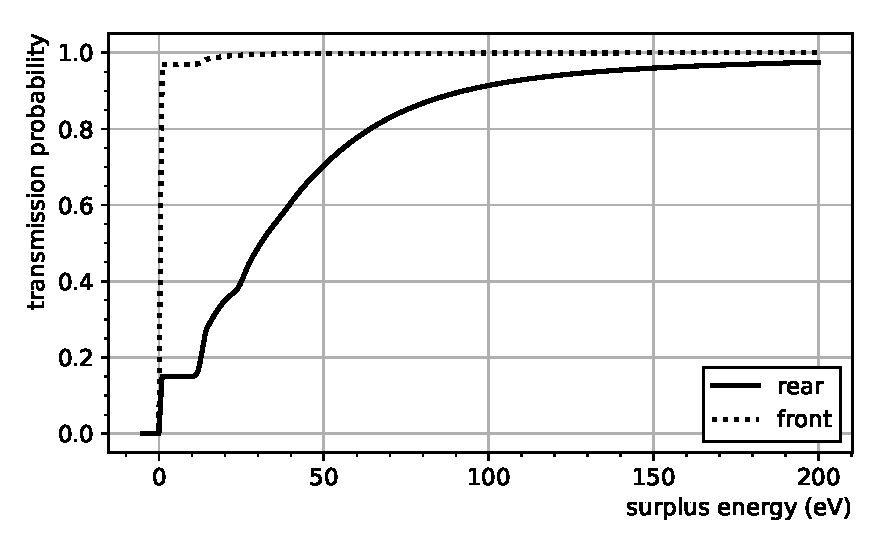
\includegraphics[width=\textwidth]{chapter/katrin/fig/response.pdf}
    \xcaption{KATRIN response function}{The response function}{as calculated by \gls{ssc}. The surplus energy denotes the difference between the starting kinetic energy $\Esource$ of a $\upbeta$ electron and the retarding energy $qU$. The response function $\bar{R}^j$ \eqref{eq:SSCresponse} is depicted for electrons starting at the rear and front of the \gls{wgts}.}
    \label{fig:response}
\end{figure}
The detected counts $N$ \eqref{eq:nonAveragedCounts} depend on the starting pitch angle $\thetaSource$ of the $\upbeta$ electrons. They have to be averaged over $\thetaSource$. The corresponding integral can be swapped with the sum over the \gls{wgts} slices and the integral over the energy and propagates to the response term
\begin{align}
\label{eq:SSCcounts}
\bar{N}(qU) \propto \sum_{j=1}^S N_T^j
\int_{qU}^{E_0}
    \left(\frac{\d \Gamma(\Esource)}{ \d \Esource}\right) \cdot
    \frac{1}{1-\cos\thetaMax^j}
    \int_{0}^{\thetaMax^j}
        R^j(\Esource, qU, \thetaSource) 
        \sin\thetaSource \d \thetaSource
\d \Esource
\fullstop
\end{align}
Here $N_T^j$ denotes the number of tritium molecules in a \gls{wgts} slice $j$. The response function $R^j$ (\ref{eq:nonAveragedResponse}) can be averaged as
\begin{equation}
\begin{split}
    \bar{R}^j(\Esource,qU) &= 
    \frac{1}{1-\cos\thetaMax^j}
    \int_{0}^{\thetaMax^j}
        R^j(\Esource, qU, \thetaSource) 
    \sin\thetaSource \d \thetaSource \\ &=
    \int_0^{\Esource}
        \sum_{l=1}^{N}
            \frac{1}{1-\cos\thetaMax^j}
            \int_{0}^{\thetaMax^j}
            \mathcal{T}^j(\Esource-\epsilon, qU, \thetaSource) \cdot
            P^j_l(\thetaSource)
            \sin\thetaSource \d \thetaSource
            f_l(\epsilon)
    \d \epsilon
    \fullstop
\end{split}
\end{equation}
The transmission function $\mathcal{T}^j$ \eqref{eq:transmission} is a step function. Assuming that $\thetaMax^j$ \eqref{eq:thetaMax} is always greater than the transmission angle $\thetaTransPure$ \eqref{eq:transmissionPitchAngle}, the upper integral boundary changes which yields the averaged response function
\begin{equation}
    \label{eq:slimResponse}
    \bar{R}^j(\Esource, qU) =
    \int_0^{\Esource}
        \sum_{l=1}^{N}
            \int_{0}^{\thetaTransPure(\Esource-\epsilon, qU)}
            \frac{
                \sin\thetaSource \cdot P^j_l(\thetaSource)
            }{
                1-\cos\thetaMax^j
            }
            \d \thetaSource
            f_l(\epsilon)
    \d \epsilon
    \fullstop
\end{equation}
The averaged response function $\bar{R}^j$ is depicted in figure \ref{fig:response}. Its formula \eqref{eq:slimResponse} can be rewritten to match the form of the formula for the non-averaged response function \mbox{$R^j$ \eqref{eq:nonAveragedResponse}}. Therefore, the averaged scattering probabilities $\bar{P}^j_l$ \eqref{eq:averagedScatProbs} are used and the factor $1 = \bar{P}^j_l / \bar{P}^j_l$ is inserted in equation \eqref{eq:slimResponse}:
\begin{align}
    \label{eq:implementedResponse}
    \bar{R}^j(\Esource, qU) &=
    \int_0^{\Esource}
        \sum_{l=1}^{N}
            \underbrace{
                \int_{0}^{\thetaTransPure(\Esource-\epsilon, qU)}
                \frac{
                    \sin\thetaSource \cdot P^j_l(\thetaSource)
                }{
                    (1-\cos\thetaMax^j) \cdot \bar{P}^j_l
                }
                \d \thetaSource
            }_{
                T^{j,\star}(\Esource-\epsilon, qU)
            } \cdot 
            \bar{P}^j_l \cdot
            f_l(\epsilon)
    \d \epsilon \\ &=
    \int_0^{\Esource}
        \sum_{l=1}^{N}
            T^{j,\star}(\Esource-\epsilon, qU) \cdot 
            \bar{P}^j_l \cdot
            f_l(\epsilon)
    \d \epsilon
    \label{eq:SSCresponse}
    \fullstop
\end{align}
Note that the non-averaged response function $R^j$ \eqref{eq:nonAveragedResponse} has the same form as the averaged one $\bar{R}^j$ \eqref{eq:SSCresponse} if the non-averaged transmission function $\mathcal{T}^j$ \eqref{eq:transmission} is replaced by the modified transmission function $T^{j,\star}$ and the non-averaged scattering probabilities $P^j_l$ (\ref{eq:scatProbs}) by the averaged ones $\bar{P}^j_l$ \eqref{eq:averagedScatProbs}.

Note further that albeit equation (\ref{eq:slimResponse}) and equation (\ref{eq:SSCresponse}) are analytically equal, they are not equal implementation-wise. Currently the implementation of the response function follows equation (\ref{eq:SSCresponse}). One one hand, equation (\ref{eq:slimResponse}) is more ``light-weight'' as it does not use the averaged scattering probabilities. In the future it might be beneficial to alter the implementation to simplify the program structure and cut down on the number of calculations. On the other hand, equation \eqref{eq:implementedResponse} allows the exchange of implementations for the transmission function whereas equation \eqref{eq:slimResponse} only allows to exchange the implementation of the response function as a whole.

\subsection{Reconciliation}
The predicted counts for a retarding energy of $qU$ when measuring a duration $t(qU)$ are
\begin{equation}
	\label{eq:countsSCCFinal}
	\bar{N}(qU) = t(qU) \cdot \detEff \cdot \left(
		\As \cdot
		 \sum_{j}
			N_T^j \cdot
			\int_{qU}^{E_0} 
				\left(\frac{\d \Gamma(\Esource)}{ \d \Esource}\right) \cdot 
				\bar{R}^j(\Esource, qU) 
			\d \Esource +
			\Rbg
		\right)
	\fullstop
\end{equation}
Here, $\As=1$ is a normalization factor, $\detEff \in [0,1]$ the detector efficiency, the sum goes over all source slices, $N_T^j$ is the number of tritium molecules in the $j$th source slice, $\left(\d \Gamma(\Esource) / \d \Esource \right)$ is the differential rate from \eqref{eq:diffRate}, $\bar{R}^j(\Esource, qU)$ is the response function from \eqref{eq:SSCresponse} and $\Rbg$ is the rate of background events.

\subsection{Amendments}
Equation \eqref{eq:countsSCCFinal} is a scaffold for an analytic model of the counts measured by the KATRIN detector. Modifications of isolated terms can consider further effects. Selected examples are:
\begin{itemize}
    \item \textbf{Doppler effect:} Gas flow and temperature move the tritium molecules and hence, smear the kinetic energy distribution of $\upbeta$ electrons. This can be modelled by convolving the differential rate $\d \Gamma / \d E$ \eqref{eq:diffRate} with a Maxwellian distribution or by applying corrections to the final energy states of the decaying molecules.
    \item \textbf{Plasma potential:} Space charges, respectively a plasma, forms within the \gls{wgts} due to the tritium decay. Electrons passing through space charges might either gain or loose energy. In a segmented \gls{wgts} volume, this is implemented by using an effective retarding energy corrected for the plasma potential $V^j$ in the slice $j$
    \begin{equation}
        qU \rightarrow qU^j_\mathrm{eff} = qU - V^j
    \end{equation} 
    when calculating the response function $\bar{R}^j$ \eqref{eq:SSCresponse}. Note that this is equivalent to using the starting potential $\Usource$ in the transmission energy $\EtransPure$ \eqref{eq:transmissionEnergy}.
    \item \textbf{Further discretization of the \gls{wgts} volume:} The \gls{ssc} software allows to discretize the \gls{wgts} not only into slices, but also to subdivide the slices further into rings and the rings into segments. This enables an arbitrary spacial binning for \gls{wgts} properties such as the magnetic field or gas density. Then, additionally, the retarding energy $qU \rightarrow qU^j$, the maximum magnetic field strength  along the beam line $\Bmax \rightarrow \Bmax^j$, the magnetic field strength in the analyzing plane $\Bana \rightarrow \Bana^j$ and the detector efficiency $\epsilon_\mathrm{det} \rightarrow \epsilon_\mathrm{det}^j$ become subject to discretization because they exhibit a radial dependency. Furthermore, the \gls{wgts} can be subdivided into volumes that map onto a specific detector pixel due to magentic guidance. This enables pixel-wise modelling of electron counts.
\end{itemize}